% THIS IS SIGPROC-SP.TEX - VERSION 3.1
% WORKS WITH V3.2SP OF ACM_PROC_ARTICLE-SP.CLS
% APRIL 2009
%
% It is an example file showing how to use the 'acm_proc_article-sp.cls' V3.2SP
% LaTeX2e document class file for Conference Proceedings submissions.
% ----------------------------------------------------------------------------------------------------------------
% This .tex file (and associated .cls V3.2SP) *DOES NOT* produce:
%       1) The Permission Statement
%       2) The Conference (location) Info information
%       3) The Copyright Line with ACM data
%       4) Page numbering
% ---------------------------------------------------------------------------------------------------------------
% It is an example which *does* use the .bib file (from which the .bbl file
% is produced).
% REMEMBER HOWEVER: After having produced the .bbl file,
% and prior to final submission,
% you need to 'insert'  your .bbl file into your source .tex file so as to provide
% ONE 'self-contained' source file.
%
% Questions regarding SIGS should be sent to
% Adrienne Griscti ---> griscti@acm.org
%
% Questions/suggestions regarding the guidelines, .tex and .cls files, etc. to
% Gerald Murray ---> murray@hq.acm.org
%
% For tracking purposes - this is V3.1SP - APRIL 2009

\documentclass{acm_proc_article-sp}
%\usepackage{[utf8x][inputenc]}
\usepackage[french,english]{babel}
\usepackage[utf8]{inputenc}
\newcommand{\subparagraph}{}
\usepackage{titlesec}
\setcounter{secnumdepth}{4}


\titleformat{\paragraph}
{\normalfont\normalsize\bfseries}{\theparagraph}{1em}{}
\titlespacing*{\paragraph}
{0pt}{3.25ex plus 1ex minus .2ex}{1.5ex plus .2ex}
\begin{document}

\title{An Extendable Python Library To Manipulate Sensors Coupled To The Raspberry Pi}
%\subtitle{[Extended Abstract]
%\titlenote{A full version of this paper is available as
%\textit{Author's Guide to Preparing ACM SIG Proceedings Using
%\LaTeX$2_\epsilon$\ and BibTeX} at
%\texttt{www.acm.org/eaddress.htm}}}
%
% You need the command \numberofauthors to handle the 'placement
% and alignment' of the authors beneath the title.
%
% For aesthetic reasons, we recommend 'three authors at a time'
% i.e. three 'name/affiliation blocks' be placed beneath the title.
%
% NOTE: You are NOT restricted in how many 'rows' of
% "name/affiliations" may appear. We just ask that you restrict
% the number of 'columns' to three.
%
% Because of the available 'opening page real-estate'
% we ask you to refrain from putting more than six authors
% (two rows with three columns) beneath the article title.
% More than six makes the first-page appear very cluttered indeed.
%
% Use the \alignauthor commands to handle the names
% and affiliations for an 'aesthetic maximum' of six authors.
% Add names, affiliations, addresses for
% the seventh etc. author(s) as the argument for the
% \additionalauthors command.
% These 'additional authors' will be output/set for you
% without further effort on your part as the last section in
% the body of your article BEFORE References or any Appendices.

\numberofauthors{2} %  in this sample file, there are a *total*
% of EIGHT authors. SIX appear on the 'first-page' (for formatting
% reasons) and the remaining two appear in the \additionalauthors section.
%
\author{
% You can go ahead and credit any number of authors here,
% e.g. one 'row of three' or two rows (consisting of one row of three
% and a second row of one, two or three).
%
% The command \alignauthor (no curly braces needed) should
% precede each author name, affiliation/snail-mail address and
% e-mail address. Additionally, tag each line of
% affiliation/address with \affaddr, and tag the
% e-mail address with \email.
%
% 1st. author
\alignauthor
Edivaldo M. F. de Jesus Jr\titlenote{Aluno do curso de An\'alise e Desenvolvimento de Sistemas(ADS)}\\
       \affaddr{Instituto Federal da Bahia}\\
       \affaddr{Rua Em\'idio dos Santos, S/N}\\
       \affaddr{Barbalho, Salvador Bahia}\\
       \email{juniorug@gmail.com}
% 2nd. author
\alignauthor
Manoel C. M. Neto\titlenote{Doutor em Ci\^encia da Computa\c{c}\~ao e Professor do Curso de An\'alise e Desenvolvimento de Sistemas}\\
       \affaddr{Instituto Federal da Bahia}\\
       \affaddr{Rua Em\'idio dos Santos, S/N}\\
       \affaddr{Barbalho, Salvador Bahia}\\
       \email{manoelnetom@ifba.edu.br}
}
% There's nothing stopping you putting the seventh, eighth, etc.
% author on the opening page (as the 'third row') but we ask,
% for aesthetic reasons that you place these 'additional authors'
% in the \additional authors block, viz.

\date{13 April 2015}
% Just remember to make sure that the TOTAL number of authors
% is the number that will appear on the first page PLUS the
% number that will appear in the \additionalauthors section.

\maketitle
\selectlanguage{french} 
\begin{abstract}
The convergence of radio technologies, microprocessors and personal digital electronic devices is leading to the concept of ubiquitous computing in which intelligent, mobile and stationary devices, coordinate with each other to provide for users immediate and universal access to new services transparently, aimed at increasing human capabilities. This work aims to define, implement and validate the design and implementation of an extensible Python library for manipulating sensors / actuators coupled to the Raspberry Pi using the raspberry-GPIO-python module. The library uses the Abstract Factory pattern to ensure that sensors / actuators and events from the same family being used in conjunction with guaranteed way. On other platforms, such as Arduino, the APIs provide libraries that encapsulate the complexity of implementation and offer only the interface to use. These libraries do not yet exist formally for those who want to use Pyton as development language applied to the Raspberry Pi. This article encourages the use of open source technologies, due to the growth of free movement of hardware, inferring the possibility of an alternative for engineers and professionals to develop their projects and provide the dissemination of knowledge. The project also presents the results obtained using some of the implemented sensors, system modeling and results described and analyzed.







%A converg\^encia das tecnologias de r\'adio, dos microprocessadores e dos dispositivos eletr\^onicos digitais pessoais est\'a levando ao conceito de Computa\c{c}\~ao Ub\'iqua no qual dispositivos inteligentes, m\'oveis e estacion\'arios, coordenam-se entre si para prover aos usu\'arios acesso imediato e universal a novos servi\c{c}os, de forma transparente, que visam aumentar as capacidades humanas. Este trabalho  tem como objetivo definir, implementar e validar o projeto e implementa\c{c}\~ao de uma biblioteca Python extens\'ivel para manipular sensores / atuadores acoplados ao Raspberry Pi usando o m\'odulo raspberry-gpio-python. A biblioteca utiliza o Padr\~ao Abstract Factory para garantir que sensores/atuadores e eventos de mesma fam\'ilia sejam usados em conjunto de forma garantida. Em outras plataformas, como no Arduino, as APIs oferecem bibliotecas que encapsulam a complexidade de implementa\c{c}\~ao e oferecem apenas a interface para o uso. Essas bibliotecas ainda n\~ao existem formalmente para quem quer usar Pyton como linguagem de desenvolvimento aplicada ao Raspberry Pi. Este artigo incentiva o uso de tecnologias de c\'odigo aberto, devido ao crescimento da livre circula\c{c}\~ao de hardware, inferindo a possibilidade de uma alternativa para engenheiros e profissionais para desenvolver seus projetos e fornecem a dissemina\c{c}\~ao do conhecimento. O projeto apresenta tamb\'em os resultados obtidos utilizando alguns dos sensores implementados, a modelagem do sistema e os resultados obtidos descritos e analisados.

%This paper provides a sample of a \LaTeX\ document which conforms to
%the formatting guidelines for ACM SIG Proceedings.
%It complements the document \textit{Author's Guide to Preparing
%ACM SIG Proceedings Using \LaTeX$2_\epsilon$\ and Bib\TeX}. This
%source file has been written with the intention of being
%compiled under \LaTeX$2_\epsilon$\ and BibTeX.

%The developers have tried to include every imaginable sort
%of ``bells and whistles", such as a subtitle, footnotes on
%title, subtitle and authors, as well as in the text, and
%every optional component (e.g. Acknowledgments, Additional
%Authors, Appendices), not to mention examples of
%equations, theorems, tables and figures.

%To make best use of this sample document, run it through \LaTeX\
%5and BibTeX, and compare this source code with the printed
%output produced by the dvi file.
\end{abstract}

\keywords{ACM proceedings, \LaTeX, text tagging} % NOT required for Proceedings
\selectlanguage{english} 
\section{Introduction}

\section{Paper Structure}

\section{THEORETICAL BACKGROUND}

\subsection{General Context}

\subsection{Mobile Computing}

\subsection{Pervasive Computing}

\subsection{Ubiquitous Computing}

\subsection{Internet of Things}

\subsection{Hardware}

\subsubsection{Sensors and Actuators}

\subsubsection{Arduino}

\paragraph{Features}

\paragraph{Digital Inputs}

\paragraph{Analog Inputs}

\paragraph{Digital outputs}

\paragraph{Special Pins}

\subsubsection{Raspberry Pi}

\paragraph{General Purpose Input/Output}

\subsubsection{WiringPi}

\subsection{raspberry-gpio-python}


\section{Correlated Work}

\section{Application}

\subsubsection{Method/Methodology}

\subsection{Architecture}

\subsection{tests}


\section{Results Obtained}


\section{Future Work}



\subsubsection{Display Equations}
\begin{equation}\lim_{n\rightarrow \infty}x=0\end{equation}
\begin{displaymath}\sum_{i=0}^{\infty} x + 1\end{displaymath}
\begin{equation}\sum_{i=0}^{\infty}x_i=\int_{0}^{\pi+2} f\end{equation}

\subsection{Citations}

\subsection{Tables}

\begin{table}
\centering
\caption{Frequency of Special Characters}
\begin{tabular}{|c|c|l|} \hline
Non-English or Math&Frequency&Comments\\ \hline
\O & 1 in 1,000& For Swedish names\\ \hline
$\pi$ & 1 in 5& Common in math\\ \hline
\$ & 4 in 5 & Used in business\\ \hline
$\Psi^2_1$ & 1 in 40,000& Unexplained usage\\
\hline\end{tabular}
\end{table}


\begin{table*}
\centering
\caption{Some Typical Commands}
\begin{tabular}{|c|c|l|} \hline
Command&A Number&Comments\\ \hline
\texttt{{\char'134}alignauthor} & 100& Author alignment\\ \hline
\texttt{{\char'134}numberofauthors}& 200& Author enumeration\\ \hline
\texttt{{\char'134}table}& 300 & For tables\\ \hline
\texttt{{\char'134}table*}& 400& For wider tables\\ \hline\end{tabular}
\end{table*}
% end the environment with {table*}, NOTE not {table}!

\subsection{Figures}

\begin{figure}
\centering
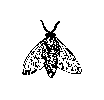
\epsfig{file=fly.eps}
\caption{A sample black and white graphic (.eps format).}
\end{figure}

\begin{figure}
\centering
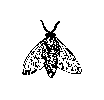
\epsfig{file=fly.eps, height=1in, width=1in}
\caption{A sample black and white graphic (.eps format)
that has been resized with the \texttt{epsfig} command.}
\end{figure}


\subsection{Theorem-like Constructs}


\subsection*{A {\secit Caveat} for the \TeX\ Expert}

\section{Conclusions}
%\end{document}  % This is where a 'short' article might terminate

%ACKNOWLEDGMENTS are optional
\section{Acknowledgments}
This section is optional; it is a location for you
to acknowledge grants, funding, editing assistance and
what have you.  In the present case, for example, the
authors would like to thank Gerald Murray of ACM for
his help in codifying this \textit{Author's Guide}
and the \textbf{.cls} and \textbf{.tex} files that it describes.

%
% The following two commands are all you need in the
% initial runs of your .tex file to
% produce the bibliography for the citations in your paper.
\bibliographystyle{abbrv}
\bibliography{sigproc}  % sigproc.bib is the name of the Bibliography in this case
% You must have a proper ".bib" file
%  and remember to run:
% latex bibtex latex latex
% to resolve all references
%
% ACM needs 'a single self-contained file'!
%
%APPENDICES are optional
%\balancecolumns
\appendix
%Appendix A
\section{Headings in Appendices}
The rules about hierarchical headings discussed above for
the body of the article are different in the appendices.
In the \textbf{appendix} environment, the command
\textbf{section} is used to
indicate the start of each Appendix, with alphabetic order
designation (i.e. the first is A, the second B, etc.) and
a title (if you include one).  So, if you need
hierarchical structure
\textit{within} an Appendix, start with \textbf{subsection} as the
highest level. Here is an outline of the body of this
document in Appendix-appropriate form:
\subsection{Introduction}
\subsection{The Body of the Paper}
\subsubsection{Type Changes and  Special Characters}
\subsubsection{Math Equations}
\paragraph{Inline (In-text) Equations}
\paragraph{Display Equations}
\subsubsection{Citations}
\subsubsection{Tables}
\subsubsection{Figures}
\subsubsection{Theorem-like Constructs}
\subsubsection*{A Caveat for the \TeX\ Expert}
\subsection{Conclusions}
\subsection{Acknowledgments}
\subsection{Additional Authors}
This section is inserted by \LaTeX; you do not insert it.
You just add the names and information in the
\texttt{{\char'134}additionalauthors} command at the start
of the document.
\subsection{References}
Generated by bibtex from your ~.bib file.  Run latex,
then bibtex, then latex twice (to resolve references)
to create the ~.bbl file.  Insert that ~.bbl file into
the .tex source file and comment out
the command \texttt{{\char'134}thebibliography}.
% This next section command marks the start of
% Appendix B, and does not continue the present hierarchy
\section{More Help for the Hardy}
The acm\_proc\_article-sp document class file itself is chock-full of succinct
and helpful comments.  If you consider yourself a moderately
experienced to expert user of \LaTeX, you may find reading
it useful but please remember not to change it.
\balancecolumns
% That's all folks!
\end{document}
